%\begin{enumerate}[1.]
%\numberwithin{equation}{\thesubsection.enumi}

%\begin{enumerate}[label=\arabic*.,ref=\thesection]
\renewcommand{\theequation}{\theenumi}
\begin{enumerate}[label=\arabic*.,ref=\thesubsection.\theenumi]
%\begin{enumerate}[label=\arabic*.,ref=\thesubsection.\theenumi]
%\numberwithin{equation}{subsection}

%\begin{enumerate}[label=\arabic*.,ref=\thesubsection.\theenumi]
%\begin{enumerate}[label=\thesection.\arabic*,ref=\thesection.\theenumi]

%\numberwithin{equation}{enumi}
\item Find the distance between 
\begin{align}
\vec{P} = \myvec{-2\\4}, \vec{Q} = \myvec{3\\-5}
\end{align}
%Mark on a diagram the points $\myvec{-2,4}, \myvec{3,-5}$ and find the distance between them.

%
\item
Find the length of $PQ$ for
\begin{enumerate}
\item $\vec{P}=\myvec{-1\\1}$ and $\vec{Q}=\myvec{2\\-1}$;
\item $\vec{P}=\myvec{4\\3}$ and $\vec{Q}=\myvec{-2\\2}$;
\item $\vec{P}=\myvec{a\\b}$ and $\vec{Q}=\myvec{-b\\a}$.
\end{enumerate}

\item Using direction vectors, show that  $\myvec{2\\1}, \myvec{4\\7}, \myvec{5\\4}$ and $\myvec{1\\4}$ are the vertices of a parallelogram.
\item Using Baudhayana's theorem, show that the points $\myvec{-3\\-4}, \myvec{2\\6}$ and $\myvec{-6\\10}$  are the vertices of a right-angled
traingle.  Repeat using orthogonality.
\item Plot the points $\myvec{0\\2},\myvec{1\\1},\myvec{4\\4}\text{ and }\myvec{3\\5}$ and prove that they are the vertices of a rectangle.
\item Show that $\vec{B}=\myvec{-2\\-2},\vec{A}=\myvec{-1\\2}\text{ and }\vec{C}=\myvec{3\\1}$ are the vertices of an isosceles triangle.
\item In the last question, find the distance of the vertex $\vec{A}$ of the triangle from the middle point of the base $BC$.
\item Prove that the points $\myvec{-1\\0}$, $\myvec{0\\3}$, $\myvec{3\\2}$ and $\myvec{2\\-1}$ are the vertices of a square.
\item Prove that the points $\vec{A}=\myvec{-1\\0}$, $\vec{B}=\myvec{3\\1}$, $\vec{C}=\myvec{2\\2}$  and $\vec{D}=\myvec{-2\\1}$ are the vertices of a parallelogram.  Find $\vec{E},\vec{F},\vec{G},\vec{H}$, the mid points of $AB, BC, CD, AD$ respectively.  Show that EG and FH bisect each other.
\item Prove that the points $\myvec{21\\-2}$, $\myvec{15\\10}$, $\myvec{-5\\0}$  and $\myvec{1\\-12}$ are the vertices of a rectangle, and find the
coordinates of its centre.
\item Find the lengths of the medians of the triangle whose vertices are at the points $\myvec{1\\2}$, $\myvec{0\\3}$ and $\myvec{-1\\-2}$.
\item Find the coordinates of the points that divide the line joining the points $\myvec{-35\\-20}$ and $\myvec{5\\-10}$ into four equal parts.
\item Find the coordinates of the points of trisection of the line joining the points $\myvec{-5\\5}$ and $\myvec{25\\10}$.
\item Prove that the middle point of the line joining the points $\myvec{-5\\12}$ and $\myvec{9\\-2}$ is a point of trisection of the line
joining the points $\myvec{-8\\-5}$ and $\myvec{7\\10}$.
\item The points $\myvec{8\\5}$, $\myvec{-7\\-5}$ and $\myvec{-5\\5}$ are three of the vertices of a parallelogram.  Find the coordinates of
the remaining vertex which is to be taken as opposite to $\myvec{-7\\-5}$.
\item The point $\myvec{2\\6}$ is the intesection of the diagonals of a parallelogram two of whose vertices are at the points $\myvec{7\\16}$ and $\myvec{10\\2}$.
Find the coordinates of the remaining vertices.
\item Find the area of the triangle whose vertices are the points $\myvec{2\\3}$, $\myvec{-4\\7}$ and $\myvec{5\\-2}$.  
\item Find the coordinates of  points which divide the join of $\myvec{2\\3}$, $\myvec{-4\\5}$ externally in the ratio $2:3$, and also
externally in the ratio $3:2$.
\item Prove the centroid of $\triangle ABC$ is
\begin{equation}
\vec{O}=\frac{\vec{A}+\vec{B}+\vec{C}}{3}
\end{equation}

\end{enumerate}
%\bibliography{IEEEabrv,gvv_opt}

%\subsection{Driving the Segments}
%Open the arduino software.  Check if the ports show Arduino Uno and click the appropriate button.  
\begin{problem}
%Connect the A-D pins of the 7447 IC to the pins D2-D5 of the Arduino.
%Connect the A-D pins of the 7447 IC  in Fig. \ref{fig:7447} to the GPIO pins  0-3 of the Pi shown in Figs. \ref{fig_1_3a} and \ref{fig_1_3b}.
\end{problem}	
\renewcommand{\thefigure}{\theproblem.\arabic{figure}}
\begin{figure}[!ht]
\begin{center}
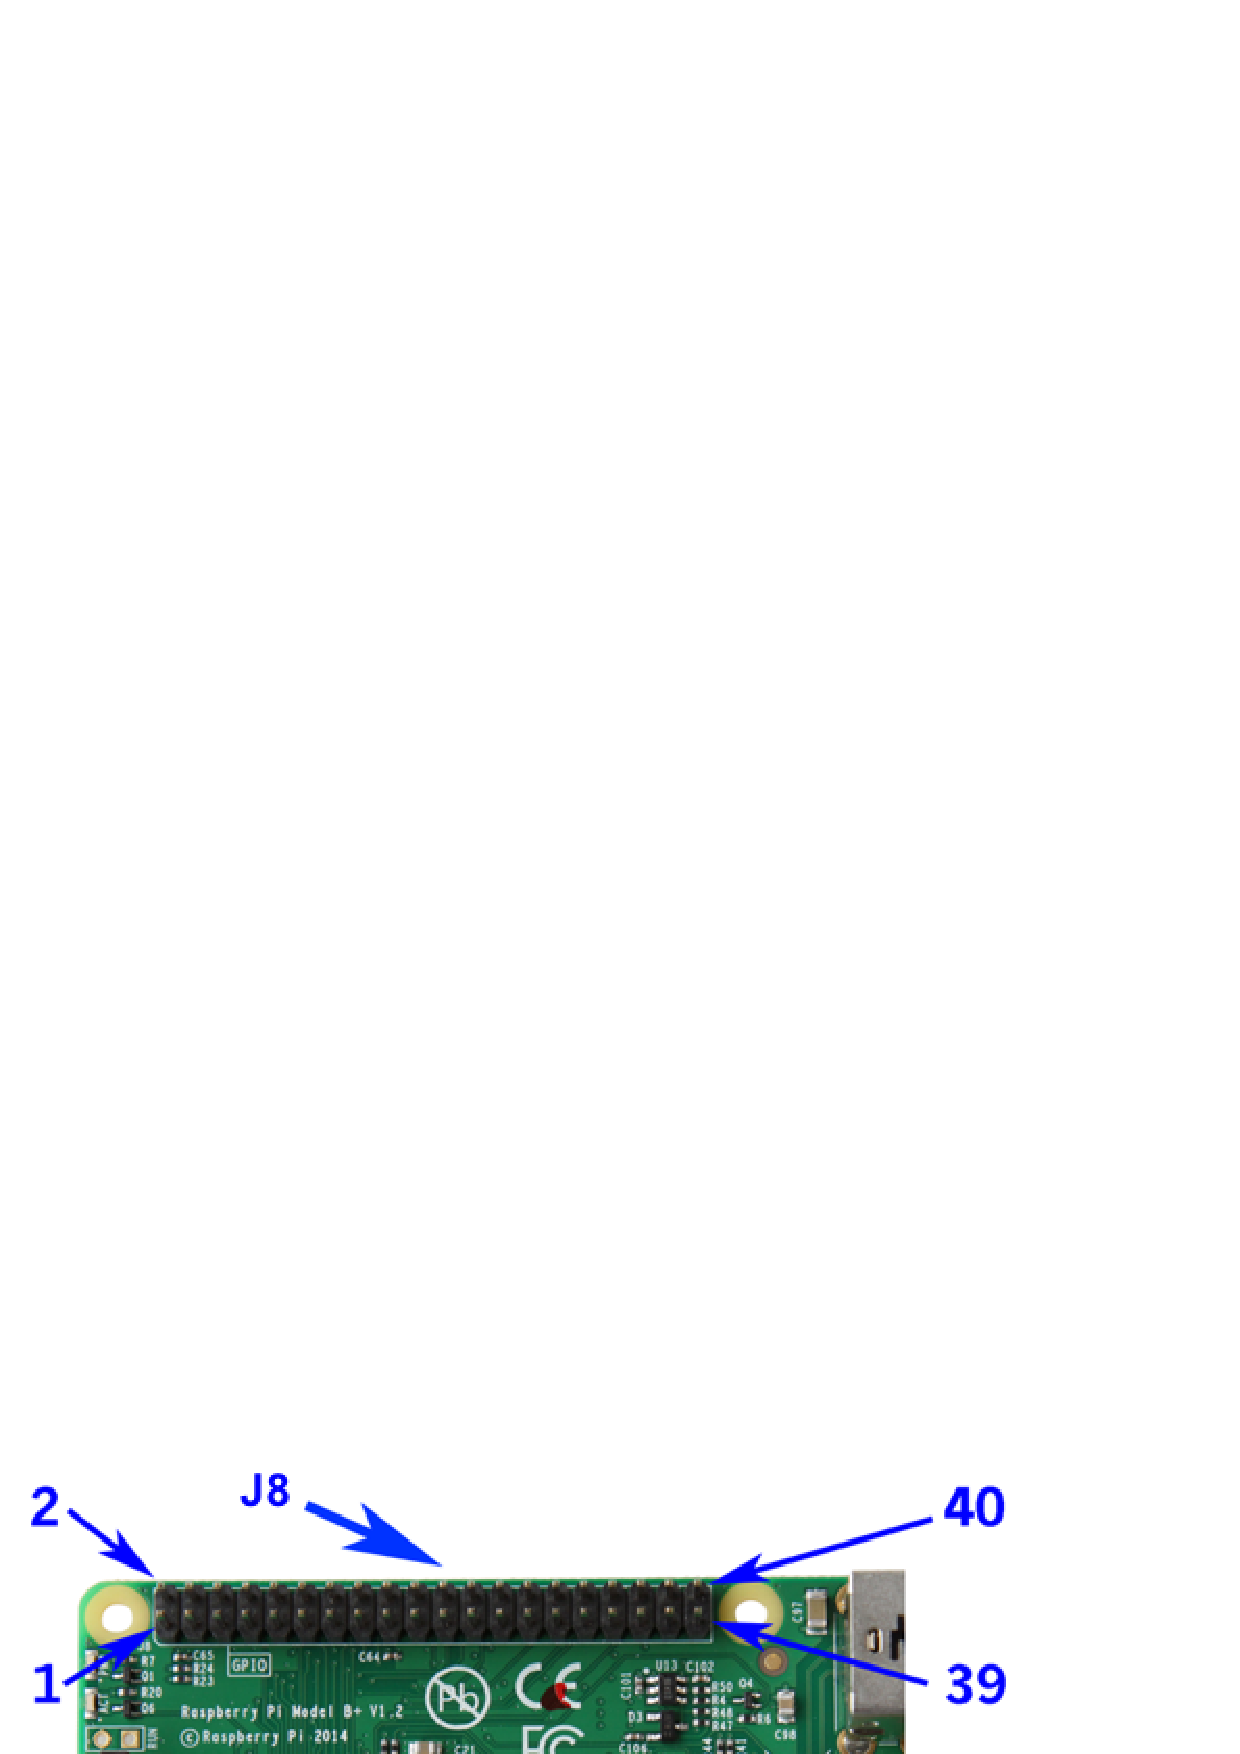
\includegraphics[width=\columnwidth]{./figs/gpio2}
\end{center}
\captionof{figure}{GPIO pin snapshot on Pi.}
\label{fig_1_3a}	
\end{figure}
%
\begin{figure}
\begin{center}
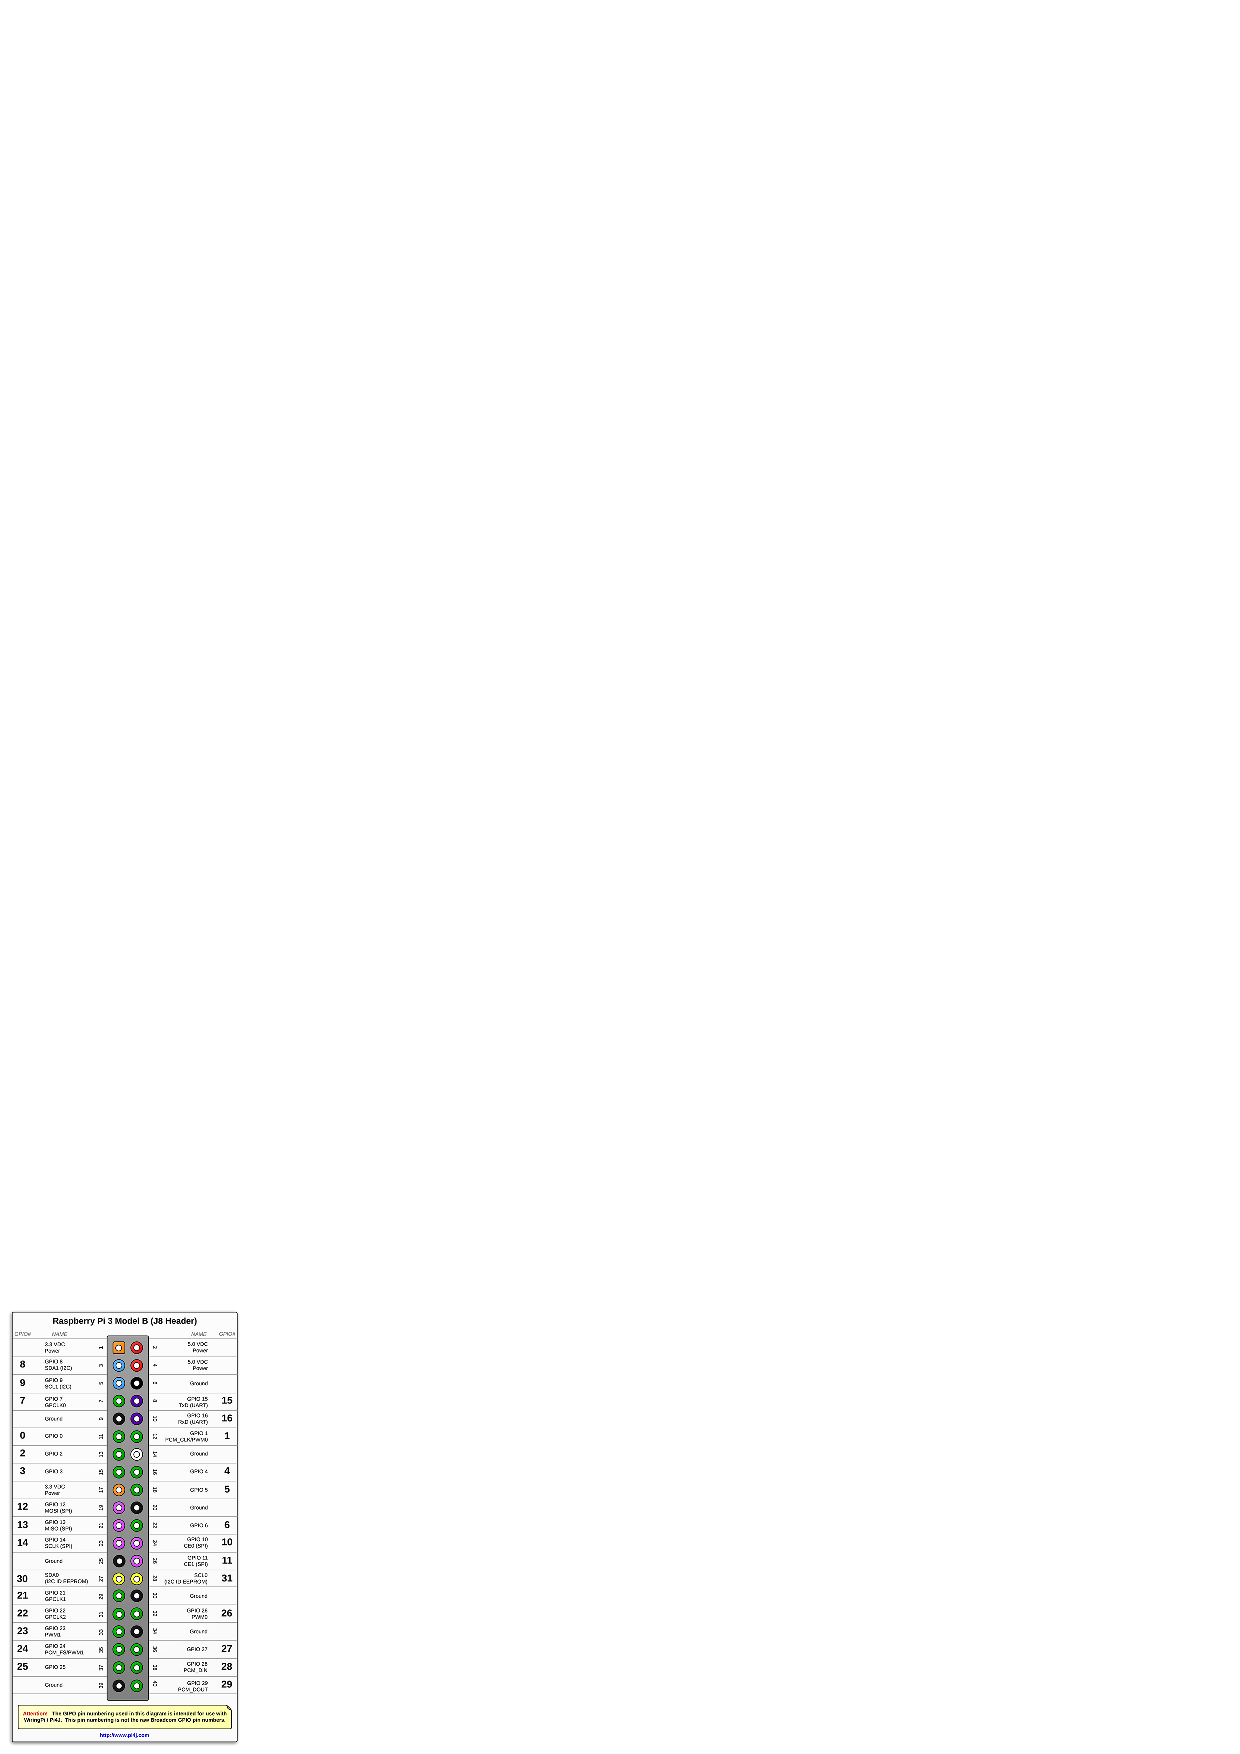
\includegraphics[width=\columnwidth]{./figs/gpio1}
\end{center}
\captionof{figure}{GPIO Wiring Pi pin configuration.}
\label{fig_1_3b}	
\end{figure}
\renewcommand{\thefigure}{\theproblem}
\begin{problem}
Connect the a-g pins of the display to the GPIO pins 0-6 of the Pi shown in \ref{fig_1_3a} and \ref{fig_1_3b}.
\end{problem}
\begin{problem}
Type the following C code and excute. What do you observe?
\end{problem}
\solution
\lstinputlisting[language=C]{./code/seven_seg_disp.c}
\begin{problem}
Now generate the numbers 0-9 by modifying the above program.
\end{problem}
\begin{problem}
Suitably modify the above program to obtain a decade counter.
\end{problem}


%\begin{problem}
%\label{prob:first_code}
%%Type the following code and execute. What do you observe?
%%\lstinputlisting[language=C]{./codes/bcd_seven.c}
%%// the setup function runs once when you press reset or power the board
int a=1,b=0,c=0,d=1,e=1,f=1,g=1;
void setup() {
    pinMode(2, OUTPUT);  
    pinMode(3, OUTPUT);
    pinMode(4, OUTPUT);
    pinMode(5, OUTPUT);
    pinMode(6, OUTPUT);
    pinMode(7, OUTPUT);
    pinMode(8, OUTPUT);            
}

// the loop function runs over and over again forever
void loop() {
  
  digitalWrite(2, a); 
  digitalWrite(3, b); 
  digitalWrite(4, c); 
  digitalWrite(5, d); 
  digitalWrite(6, e); 
  digitalWrite(7, f);     
  digitalWrite(8, g); 
}


%\end{problem}
%\begin{problem}
%Now generate the numbers 0-9 by modifying the above program.
%\end{problem}
%%
%%\newpage

%%\section{Combinational Logic}
%%
%\subsection{Counting Decoder}
	%In the  truth table in Table \ref{table:counter_decoder},  $W,X,Y,Z$ are the inputs
%and $A,B,C,D$ are the outputs. This table represents the system that increments the numbers 0-8 by 1 and resets the number 9 to 0
%%
%Note that  $D = 1$ for the inputs $0111$ and $1000$.  Using {\em boolean} logic,
%%
%\begin{equation}
%\label{bool_logic}
%D = WXYZ^{'} + W^{'}X^{'}Y^{'}Z
%\end{equation}
%%
%Note that $0111$ results in the expression $WXYZ^{'}$ and $1000$ yields $W^{'}X^{'}Y^{'}Z$. 
%%The $\&\&$ operand is used for the boolean AND (multiplication) operation, the $||$ operand is used for the OR (addition) operation and the ! operand is used for the NOT ($^{'}$) operation in Arduino code.  For example, the expression for \eqref{bool_logic} in Arudino is
%%\begin{verbatim}
%%D = (W&&X&&Y&&!Z)||(!W&&!X&&!Y&&Z);
%%\end{verbatim}

%\begin{problem}
	%\label{counter_dec}

%Write the boolean logic functions for $A,B,C$ in terms of $W,X,Y,Z$.
%\end{problem}
%%
%\input{./figs/counter_decoder}
%%
%%
%\begin{problem}
%%	\label{D_code}
%Write a program for implementing Table \ref{counter_dec}.
%%\eqref{bool_logic} in Arduino.
%\end{problem}
%%
%\solution
%%\lstinputlisting[language=C]{./codes/count_decoder.c}
%%
%%\begin{problem}
%%Modify the above program by keeping W=0,X=0,Y=0,Z=1 and A=1 and execute.  Verify that your results are consistent with Table \ref{counter_dec}.
%%\end{problem}

%\begin{problem}
%Verify if your logic is correct by observing the output on the seven segment display for different inputs.
%\end{problem}
%%
%\begin{problem}
%Connect GPIO pin 10 to the dot pin of the display and execute the following code.
%\end{problem}
%%\lstinputlisting[language=C]{./codes/blink.c}
%%
%%
%\begin{problem}
%A decade counter counts the numbers from 0-9 and then resets to 0.  Suitable modify the above programs to obtain a decade counter.
%\end{problem}

%\subsection{Display Decoder}
%%
%\begin{problem}
%Now write the truth table for the seven segment display decoder (IC 7447).  The inputs will be $A,B,C,D$ and the outputs will be $a,b,c,d,e,f,g$.
%\end{problem}
%%
%\begin{problem}
%\label{seven_seg_disp_logic}
%Obtain the logic functions for outputs $a,b,c,d,e,f,g$ in terms of the inputs $A,B,C,D$.
%\end{problem}
%\begin{problem}
%Disconnect the Pi from IC 7447 and connect the pins GPIO 0-6 in the Pi directly to the seven segment display.
%\end{problem}
%\begin{problem}
%Write a new program to implement the logic in Problem \ref{seven_seg_disp_logic} and observe the output in the display.  You have designed the logic for IC 7447!
%\end{problem}
%\begin{problem}
%Now include your counting decoder program in the  display decoder program
%and see if the display shows the consecutive number.
%\end{problem}
%A decade counter counts the numbers from 0-9 and then resets to 0.
%\begin{problem}
%Suitably modify the above program to obtain a decade counter.
%\end{problem}




%\begin{problem}
%Generate the boolean functions for the segments $a-f$ using the table in Problem \ref{bcd_ss}.  For example, the function for $a$ is obtained from the table as
%\begin{equation}
%a=\bar{D}\bar{C}\bar{B}A+\bar{D}C\bar{B}\bar{A}
%\label{boolean}
%\end{equation}
%\end{problem}
%%
%\begin{problem}
	%\label{counter_dec}
%Write functions for $A,B,C,D$ in Arduino using the following table and verify using the Arduino driven display.
		%\input{counter_decoder}
%\end{problem}
%\begin{problem}
	%Write a module for decimal to binary conversion
	%according to the example given below
	%\input{conversion}
	%%
	%$N \% 2$ gives the remainder and $N/2$ gives the quotient
%	and use it in the above code so that decimal values are given as input in the program and observed as output in the display. Note that the following code
%	\begin{verbatim}
%	a % b
%	\end{verbatim}
%	can be used to obtain the remainder when a is divided by b and
%	\begin{verbatim}
%	a/b
%	\end{verbatim}
%	gives the quotient.
%\end{problem}
 
%%
%\newpage
%\section{$M$-ary Modulation}
%\subsection{Angle Bisectors}

\begin{figure}[!h]
	\begin{center}
		
		%
\includegraphics[width=\columnwidth]{./figs/ch3_angle_bisector}
		%\vspace*{-10cm}
		\resizebox{\columnwidth}{!}{\begin{tikzpicture}
[scale=2,>=stealth,point/.style={draw,circle,fill = black,inner sep=0.5pt},]

\node (D) at (0, 0)[point,label=below :$D$] {};
\node (A) at (0, 3)[point,label=above :$A$]{};
\node (B) at (-3, 0)[point,label=below left:$B$]{};
\node (C) at (3, 0)[point,label=below right:$C$]{};
\node (O) at (0, 1.3)[point,label=below right:$O$]{};
\node (F) at (-1.1, 1.9)[point,label=above left:$F$]{};
\node (E) at (1.1, 1.9)[point,label=above right:$E$]{};

\draw (D)--(B);
\draw (B)--(A);
\draw (A)--(C);
\draw (C)--(D);
\draw [thick,dashed] (A) -- (D);
\draw [thick,dashed] (O) -- (E);
\draw [thick,dashed] (O) -- (F);
\draw (B)--(O);
\draw (C)--(O);

\tkzMarkRightAngle[size=.2](A,D,C)
\tkzMarkRightAngle[size=.15](B,F,O);
\tkzMarkRightAngle[size=.15](C,E,O);
\tkzMarkAngle[size=.4](D,B,O);
\tkzMarkAngle[size=.35](O,B,F);
\tkzMarkAngle[size=.54](E,C,O);
\tkzMarkAngle[size=.5](E,C,O);
\tkzMarkAngle[size=.6](O,C,D);
\tkzMarkAngle[size=.65](O,C,D);

\end{tikzpicture}}
	\end{center}
	\caption{Angle bisectors meet at a point}
	\label{ch3_angle_bisector}	
\end{figure}

\begin{definition}
	In Fig. \ref{ch3_angle_bisector}, $OB$ divides the  $\angle B$ into half, i.e.\begin{equation}
	\angle OBC = \angle OBA
	\end{equation}
	$OB$ is known as an angle bisector.
\end{definition}
	$OB$ and $OC$ are angle bisectors of angles $B$ and $C$. $OA$ is joined and $OD, OF$ and $OE$ are perpendiculars to sides $a,b$ and $c$.
\begin{problem}
  Show that $OD = OE = OF$.
\end{problem}
\proof In $\Delta$s $ODC$ and $OEC$,
\begin{align}
OD &= OC \sin \frac{C}{2}
\\
OE &= OC \sin \frac{C}{2} 
\\
\Rightarrow OD &=OE.
\end{align}
Similarly,
\begin{equation}
OD = OF.
\end{equation}
%
\begin{problem}
	Show that OA is the angle bisector of $\angle A$
\end{problem}
\proof In $\Delta$s $OFA$ and $OEA$,
\begin{align}
OF &= OE
\\
\Rightarrow OA \sin OAF &= OA \sin OAE \\
\Rightarrow \sin OAF &=  \sin OAE \\
\Rightarrow \angle OAF &= \angle OAE
\end{align}
which proves that $OA$ bisects $\angle A$.
{\em Conclusion:} The angle bisectors of a triangle meet at a point.


\subsection{Congruent Triangles}
%
\begin{problem}
	Show that in $\Delta$s $ODC$ and $OEC$, corresponding sides and angles are equal.
\end{problem}
\begin{definition}
	Note that    $\Delta$s $ODC$ and $OEC$ are known as congruent triangles.  To show that two triangles are congruent, it is sufficient to show that some angles and sides are equal.
\end{definition}
\begin{problem}
SSS:	Show that if the corresponding sides of three triangles are equal, the triangles are congruent.
\end{problem}
\begin{problem}
ASA:	Show that if two angles and any one side  are equal in corresponding triangles, the triangles are congruent.
\end{problem}
\begin{problem}
SAS:	Show that if two sides and the angle between them are equal in corresponding triangles, the triangles are congruent.
\end{problem}
\begin{problem}
RHS:	For two right angled triangles, if the hypotenuse and one of the sides are equal, show that the triangles are congruent.
\end{problem}
	%
%%
\subsection{Perpendicular Bisectors}
\begin{definition}
	In Fig. \ref{ch3_perp_bisector}, OD $\perp BC$ and $BD=DC$. $OD$ is defined as the perpendicular bisector of $BC$.
\end{definition}

\begin{problem}
	In Fig. \ref{ch3_perp_bisector}, show that $OA=OB=OC$.
\end{problem}
%%
%%
\begin{figure}[!h]
	\begin{center}
		
		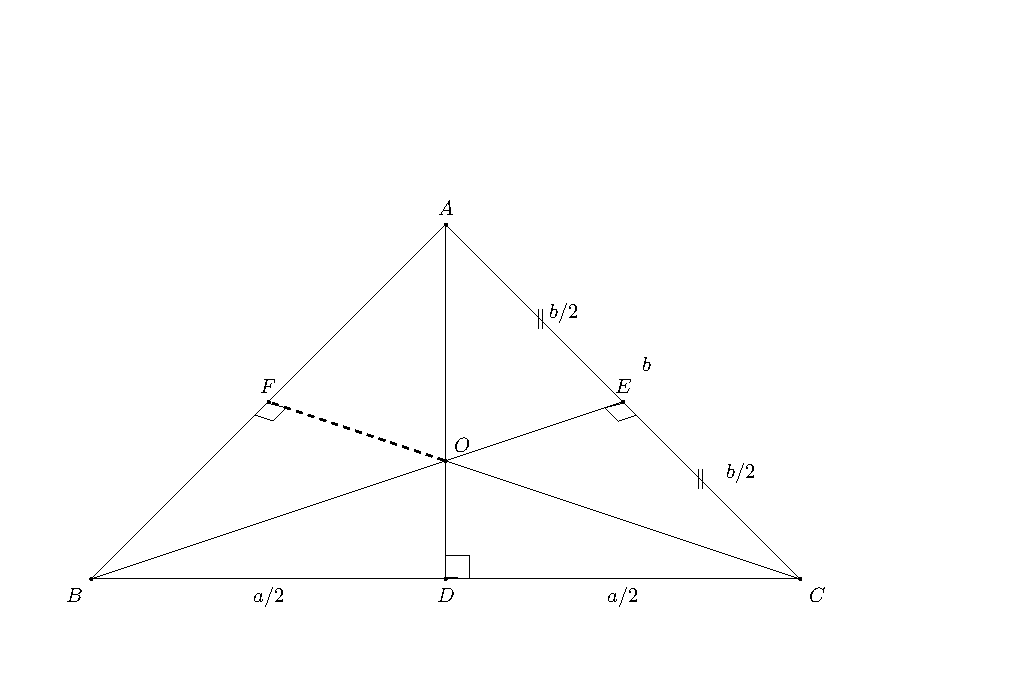
\includegraphics[width=\columnwidth]{./figs/fig_3.8.eps}
%		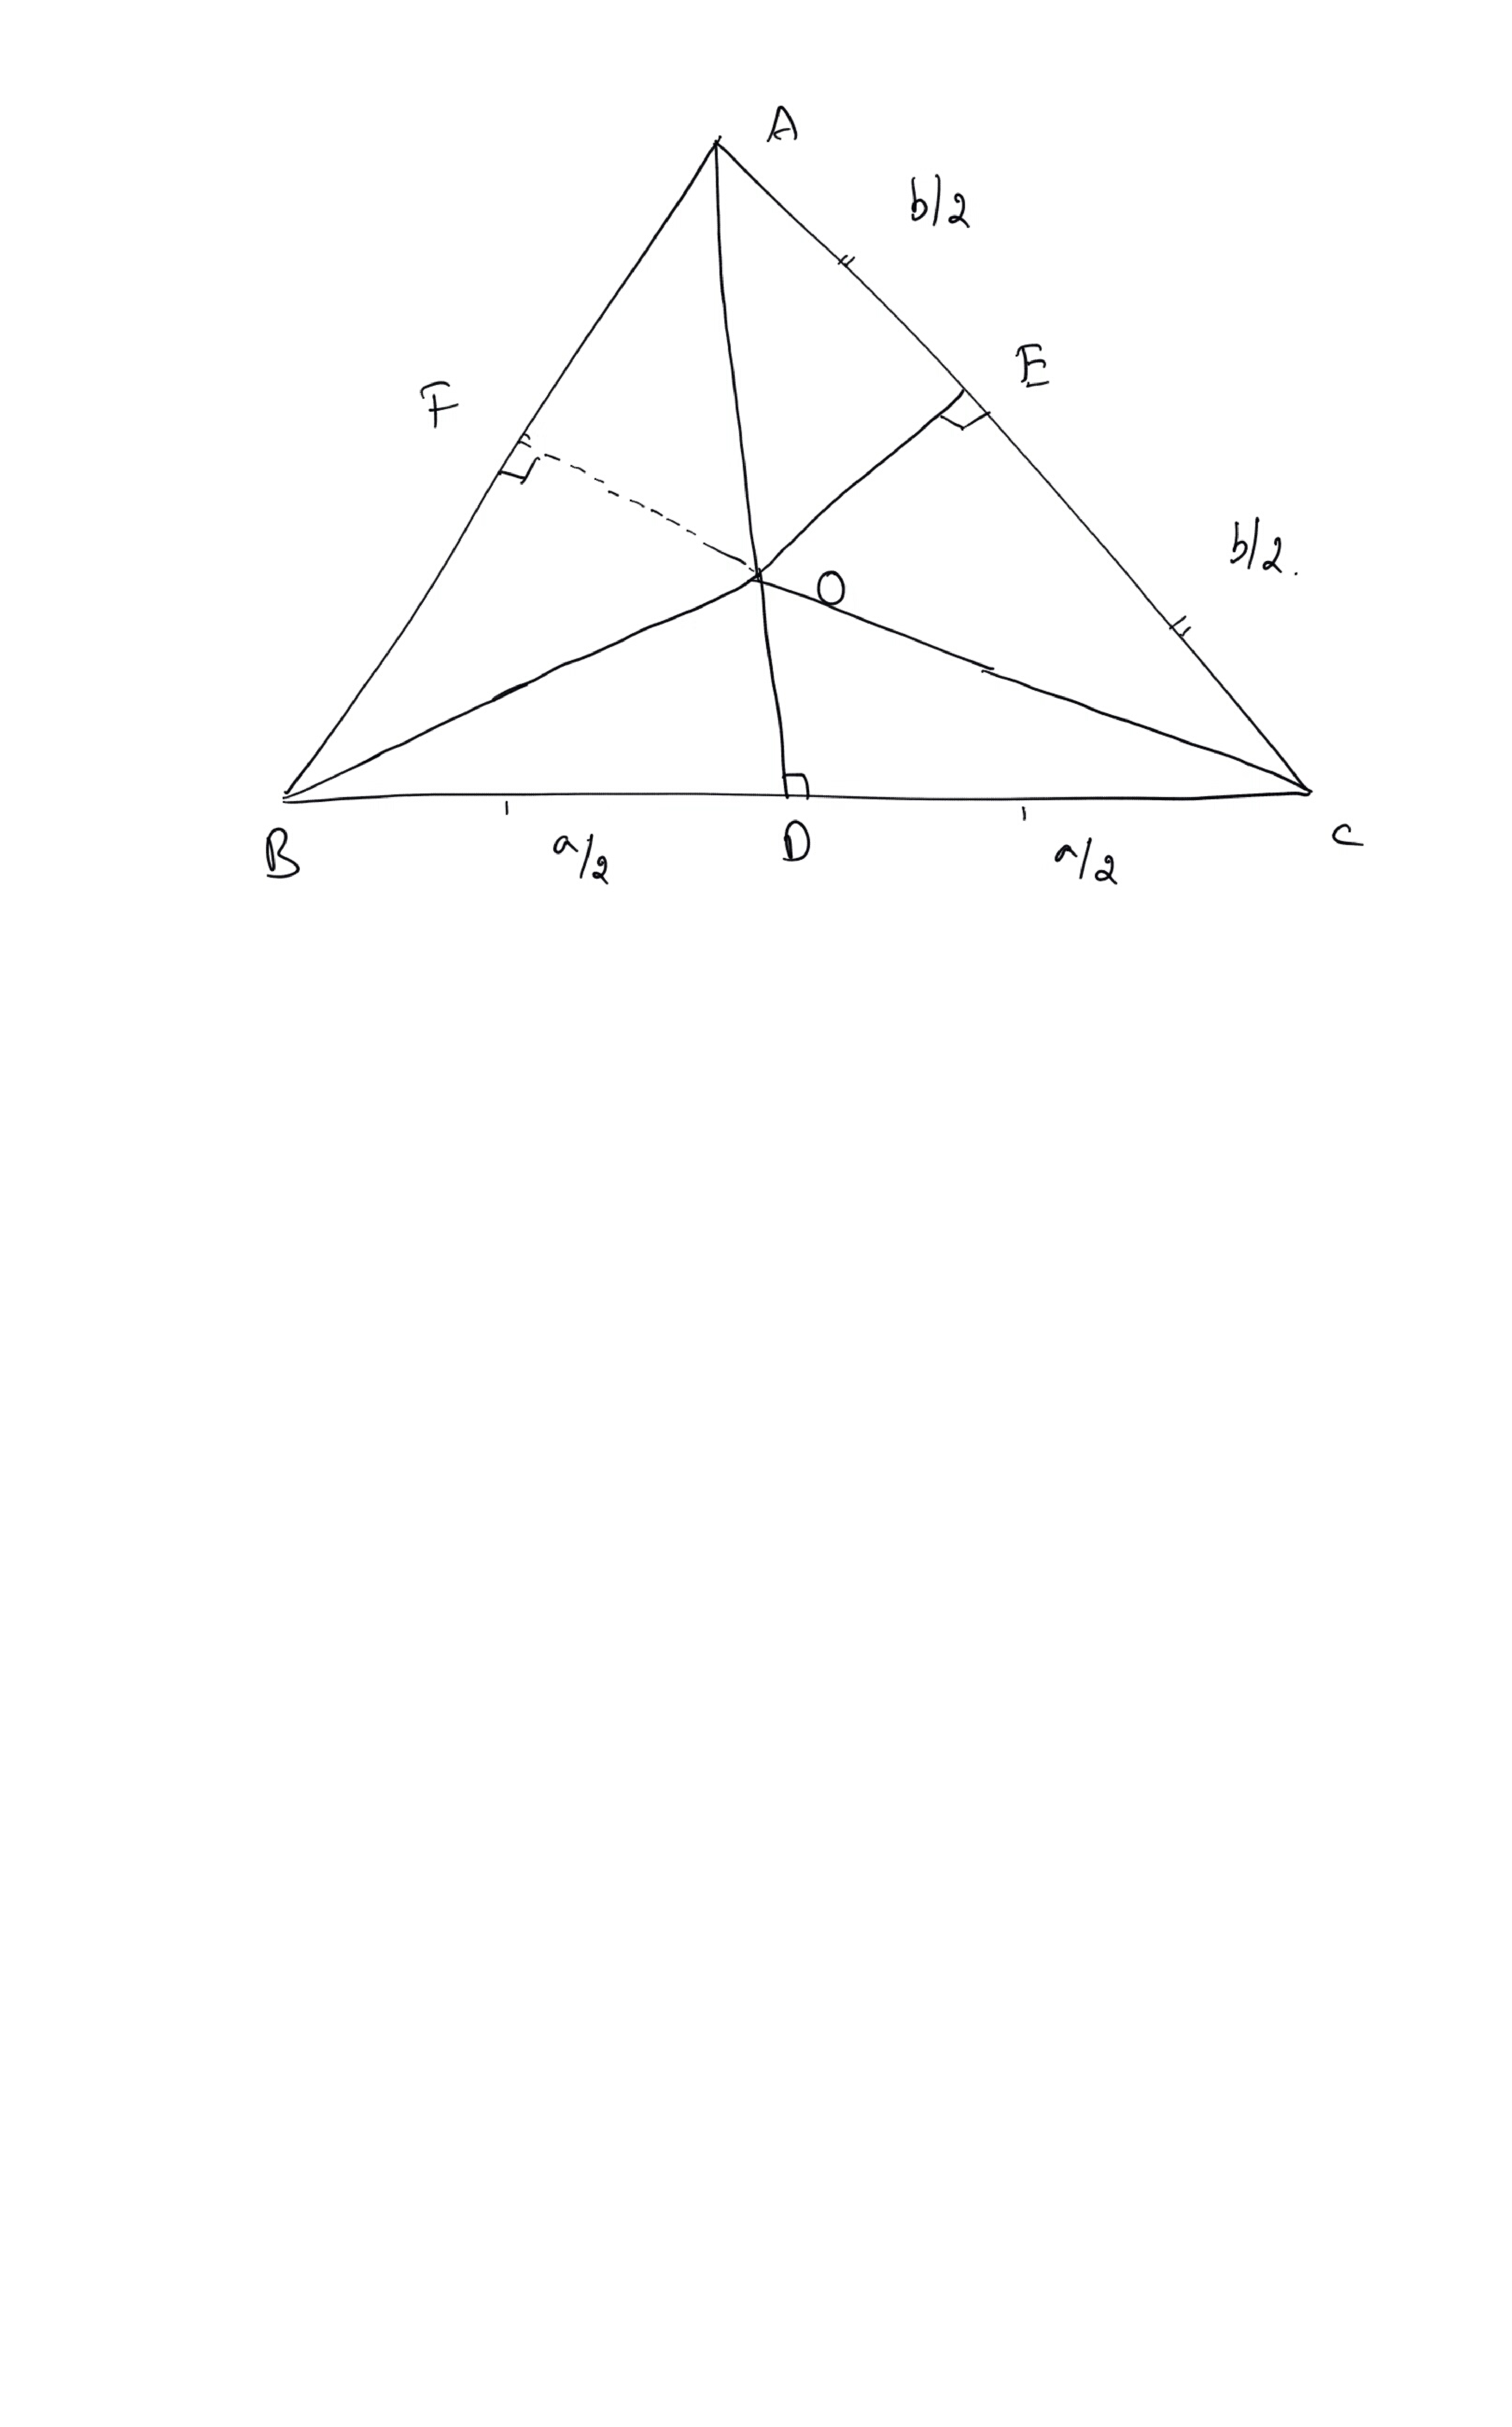
\includegraphics[width=\columnwidth]{./figs/ch3_perp_bisector}
		%\vspace*{-10cm}
%		\resizebox{\columnwidth}{!}{\documentclass{standalone}
\usepackage{tikz}
\usepackage{tkz-euclide}
\usetkzobj{all}
%\usepackage{amsmath}
\providecommand{\brak}[1]{\ensuremath{\left(#1\right)}}

\begin{document}
\begin{tikzpicture}
[scale=2,>=stealth,point/.style={draw,circle,fill = black,inner sep=0.5pt},]

\node (E) at (1.5, 1.5)[point,label=above :$E$] {};
\node (F) at (-1.5, 1.5)[point,label=above :$F$] {};
\node (A) at (0, 3)[point,label=above :$A$]{};
\node (B) at (-3, 0)[point,label=below left:$B$]{};
\node (C) at (3, 0)[point,label=below right:$C$]{};
\node (D) at (0,0)[point,label=below :$D$] {};
\node (O) at (0,1)[point,label=above right :$O$] {};


\draw (B)--(A);
\draw (A)--(C);
\draw (B)--(C);
\draw (B)--(E);
\draw (C)--(O);
\draw (A)--(D);
\draw [thick,dashed] (O) -- (F);

\node [above] at (1.7,1.7) {$b$};
\node [above] at (2.5,.75) {$b/2$};
\node [above] at (1,2.1) {$b/2$};
\node [above] at (-1.5,-0.3){$a/2$};
\node [above] at (1.5,-0.3){$a/2$};
\tkzMarkRightAngle[size=.16](B,F,O)
\tkzMarkRightAngle[size=.16](C,E,O)
\tkzMarkRightAngle[size=.2](A,D,C)
\draw   -- (4.3,1.7) node[midway] {$\parallel$};
\draw   -- (1.6,4.4) node[midway] {$\parallel$};

\end{tikzpicture}
\end{document}}
	\end{center}
	\caption{Perpendicular bisectors meet at a point}
	\label{ch3_perp_bisector}	
\end{figure}
%
\proof In $\Delta$s $ODB$ and $ODC$, using Budhayana's theorem,
%
\begin{equation}
\begin{split}
OB^2 &= OD^2 + BD^2 \\
OC^2 &= OD^2 + DC^2 
\end{split}
\end{equation}
%
Since $BD = DC = \frac{a}{2}$, $OB = OC$.  Similarly, it can be shown that $OA = OC$.  Thus, $OA=OB=OC$.
%
\begin{definition}
	In $\Delta AOB$, $OA = OB$.  Such a triangle is known as an isoceles triangle.
\end{definition}
%
\begin{problem}
	Show that $AF = BF$.
\end{problem}
\proof Trivial using Budhayana's theorem.  This shows that $OF$ is a perpendicular bisector of $AB$. 
{\em Conclusion:}  The perpendicular bisectors of a triangle meet at a point.
%
\subsection{Perpendiculars from Vertex to Opposite Side}
	%
	%
	In Fig. \ref{ch3_perp_triang}, $AD \perp BC$ and $BE \perp AC$. $CF$ passes through $O$ and meets
	$AB$ at $F$.  	
\begin{problem}
	Show that 
	\begin{align}
	OE = c \cos A \cot C
	\end{align}
\end{problem}
	\begin{figure}[!h]
		\begin{center}
			
			%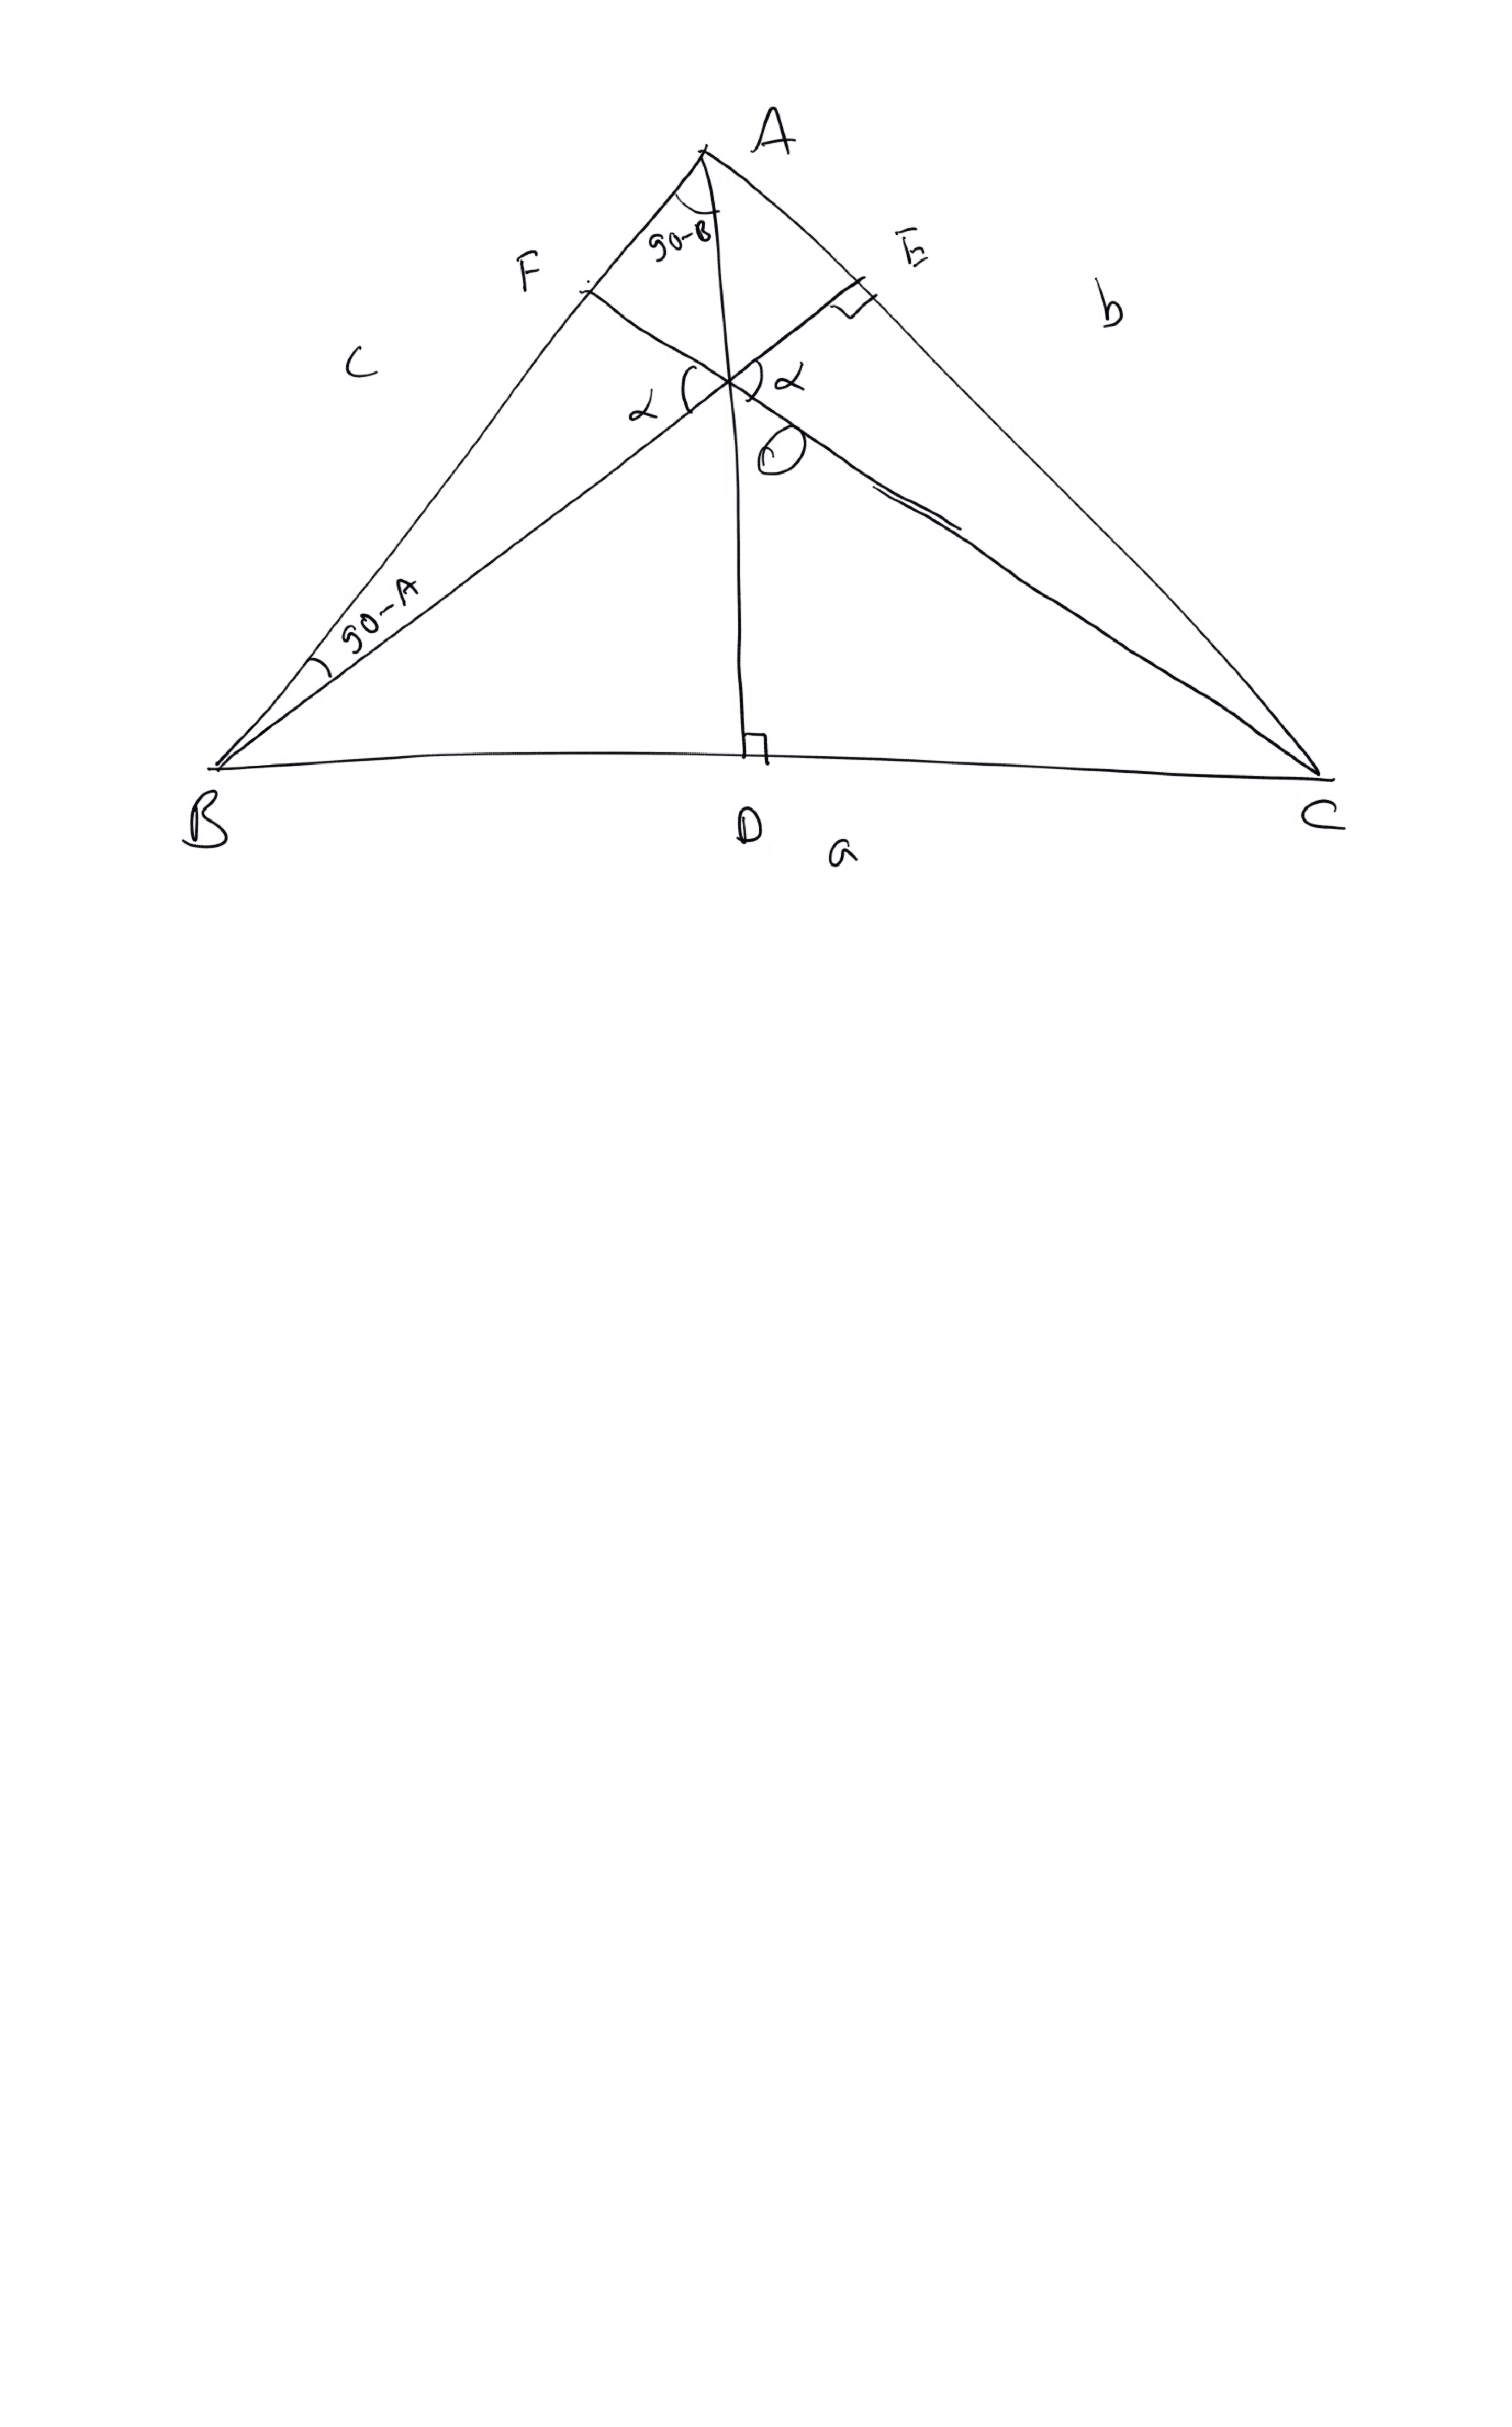
\includegraphics[width=\columnwidth]{./figs/ch3_perp_triang}
			%\vspace*{-10cm}
			\resizebox{\columnwidth}{!}{\begin{tikzpicture}
[scale=2,>=stealth,point/.style={draw,circle,fill = black,inner sep=0.5pt},]

\node (E) at (1.5, 1.5)[point,label=above :$E$] {};
\node (F) at (-1.5, 1.5)[point,label=above :$F$] {};
\node (A) at (0, 3)[point,label=above :$A$]{};
\node (B) at (-3, 0)[point,label=below left:$B$]{};
\node (C) at (3, 0)[point,label=below right:$C$]{};
\node (O) at (0,1)[point,label=above right :$O$] {};
\node (D) at (0,0)[point,label=below :$D$] {};


\draw (B)--(A);
\draw (A)--(C);
\draw (B)--(E);
\draw (C)--(F);
\draw (B)--(C);
\draw (A)--(D);

\node [below] at (0,-0.3) {$a$};
\node [above] at (-1.7,1.7) {$c$};
\node [above] at (1.7,1.7) {$b$};
\node [above] at (1,1.3) {$p$};
\node [above] at (-1,1.3) {$q$};
\node [above] at (-2.3,0.24){\rotatebox{45}{$90-A$}};
\node [above] at (-0.4,2.1) {\rotatebox{45}{$90-B$}};
\node [above] at (0.4,2.1) {\rotatebox{-45}{$90-C$}};

\tkzMarkAngle[size=.3](F,O,B);
\tkzMarkAngle[size=.3](C,O,E);
\tkzMarkAngle[size=.4](O,B,F);
\tkzMarkAngle[size=.2](F,A,O);
\tkzMarkAngle[size=.3](O,A,E);
\draw (-0.5,1) node{$\alpha$};
\draw (0.5,1) node{$\alpha$};

\end{tikzpicture}
}
		\end{center}
		\caption{Perpendiculars from vertex to opposite side meet at a point}
		\label{ch3_perp_triang}	
	\end{figure}
%
\proof In $\Delta$ s $AEB$ and $AEO$,
%
\begin{align}
AE &= c \cos A \\
OE &= AE \tan \brak{90^{\degree} - C} \brak{\because ADC \text{ is right angled}} \\
&= AE \cot C
\end{align}
%
From both the above, we get the desired result.
%
\begin{problem}
	Show that $\alpha = A$.
\end{problem}
\proof In $\Delta OEC$,
%
\begin{equation}
CE = a \cos C \brak{\because BEC \text{ is right angled}}
\end{equation}
%
Hence,
%
\begin{equation}
\begin{split}
\tan \alpha &= \frac{CE}{OE} \\
&=  \frac{a \cos C}{c \cos A \cot C} \\
&=  \frac{a \cos C \sin C}{c \cos A \cos C} \\
&= \frac{a \sin C}{c \cos A } \\
&= \frac{c \sin A}{c \cos A } \brak{\because \frac{a}{\sin A} = \frac{c}{\sin C}}\\
&= \tan A\\
\Rightarrow \alpha = A
\end{split}
\end{equation}
%
\begin{problem}
	Show that $CF \perp AB$
\end{problem}
\proof Consider triangle OFB and the result of the previous problem.  $\because$ the sum of the angles of a triangle is $180^{\degree}$, $\angle CFB = 90^{\degree}$.
{\em Conclusion: The perperdiculars from the vertex of a triangle to the opposite side meet at a point.} 
%
%\newpage
%\section{BER in Rayleigh Flat Slowly Fading Channels}
	%\subsection{Chord of a Circle}

\begin{figure}[!h]
	\begin{center}
		
		
\includegraphics[width=\columnwidth]{./figs/ch4_circle_def}
		\vspace*{-10cm}
	\end{center}
	\caption{Circle Definitions}
	\label{ch4_circle_def}	
\end{figure}
\begin{definition}
	Fig. \ref{ch4_circle_def} represents a circle.  The points in the circle are at a distance $r$ from the centre $O$.  $r$ is known as the radius.
\end{definition}

\subsection{Chords of a circle}
\begin{definition}
	In Fig. \ref{ch4_circle_def}, $A$ and $B$ are points on the circle.  The line $AB$ is known as a chord of the circle.
\end{definition}
%
%
\begin{problem}
	\label{ch4_prob_circle_subtend}
	In Fig. \ref{ch4_circle_subtend}  Show that $\angle OAB = 2\angle APB $.
\end{problem}
\begin{figure}[!h]
	\begin{center}
		
		
\includegraphics[width=\columnwidth]{./figs/ch4_circle_subtend}
		\vspace*{-10cm}
	\end{center}
	\caption{Angle subtended by chord $AB$ at the centre $O$ is twice the angle subtended at $P$. }
	\label{ch4_circle_subtend}	
\end{figure}

\proof In Fig. \ref{ch4_circle_subtend}, the triangeles $OPA$ and $OPB$ are isosceles. Hence,
%
\begin{align}
\angle OPB = \angle OBP &= \theta_1 \\
\angle OPA = \angle OAP &= \theta_2
\end{align}
%
Also, $\alpha$ and $\beta$ are exterior angles corresponding to the triangle $OPB$ and $OPA$ respectively. Hence
%
\begin{align}
\alpha &= 2\theta_1 \\
\beta &= 2\theta_2
\end{align}
%
Thus,
%
\begin{align}
\angle AOB &= \alpha + \beta \\
&= \theta_1 + \theta_2 \\
&= \angle APB
\end{align}
%
\begin{definition}
	The diameter of a circle is the chord that divides the circle into two equal parts. In Fig. \ref{ch4_circle_dia}, $AB$ is the diameter and passes through the centre $O$
\end{definition}
%
\begin{problem}
In Fig. \ref{ch4_circle_dia}, show that $\angle APB = 90^{\degree}$ .
\end{problem}
%
\begin{figure}[!h]
	\begin{center}
		
		
\includegraphics[width=\columnwidth]{./figs/ch4_circle_dia}
		\vspace*{-10cm}
	\end{center}
	\caption{Diameter of a circle.}
	\label{ch4_circle_dia}	
\end{figure}

\begin{problem}
	In Fig. \ref{ch4_chord_product}, show that 
	\begin{equation}
	\begin{split}
\angle ABD &= \angle ACD \\
\angle CAB &= \angle CDB	
	\end{split}
	\end{equation}
\end{problem}
\begin{figure}[!h]
	\begin{center}
		
		
\includegraphics[width=\columnwidth]{./figs/ch4_chord_product}
		\vspace*{-10cm}
	\end{center}
	\caption{$PA.PB = PC.PD$}
	\label{ch4_chord_product}	
\end{figure}
%
%
\proof Use Problem \ref{ch4_prob_circle_subtend}.
%
\begin{problem}
	In Fig. \ref{ch4_chord_product}, show that the triangles $PAB$ and $PBD$ are similar
\end{problem}
\proof Trivial using previous problem
\begin{problem}
	In Fig. \ref{ch4_chord_product}, show that 
	\begin{equation}
	PA.PB = PC.PD
	\end{equation}
\end{problem}
%
\proof Since triangles $PAC$ and $PBD$ are similar, 
%
\begin{align}
\frac{PA}{PD} &= \frac{PC}{PB} \\
\Rightarrow PA.PB &= PC.PD
\end{align}
%
%
\begin{definition}
	The line $PX$ in Fig. \ref{ch4_tangent_def} touches the circle at exactly one  point $P$. It is known as the tangent to the circle.
\end{definition}
%
%
\begin{problem}
	$OP$ is the perpendicular to the line $PX$ as shown in the Fig. \ref{ch4_short_dist}. Show that $OP$ is the shortest distance between the point $O$ and the line $PX$. 
\end{problem}
\proof Let $P_1$ be a point on the line $PX$. Then $OPP_1$ is a right angled triangle.  Using Budhayana's theorem,
%
\begin{figure}[!h]
	\begin{center}
		
		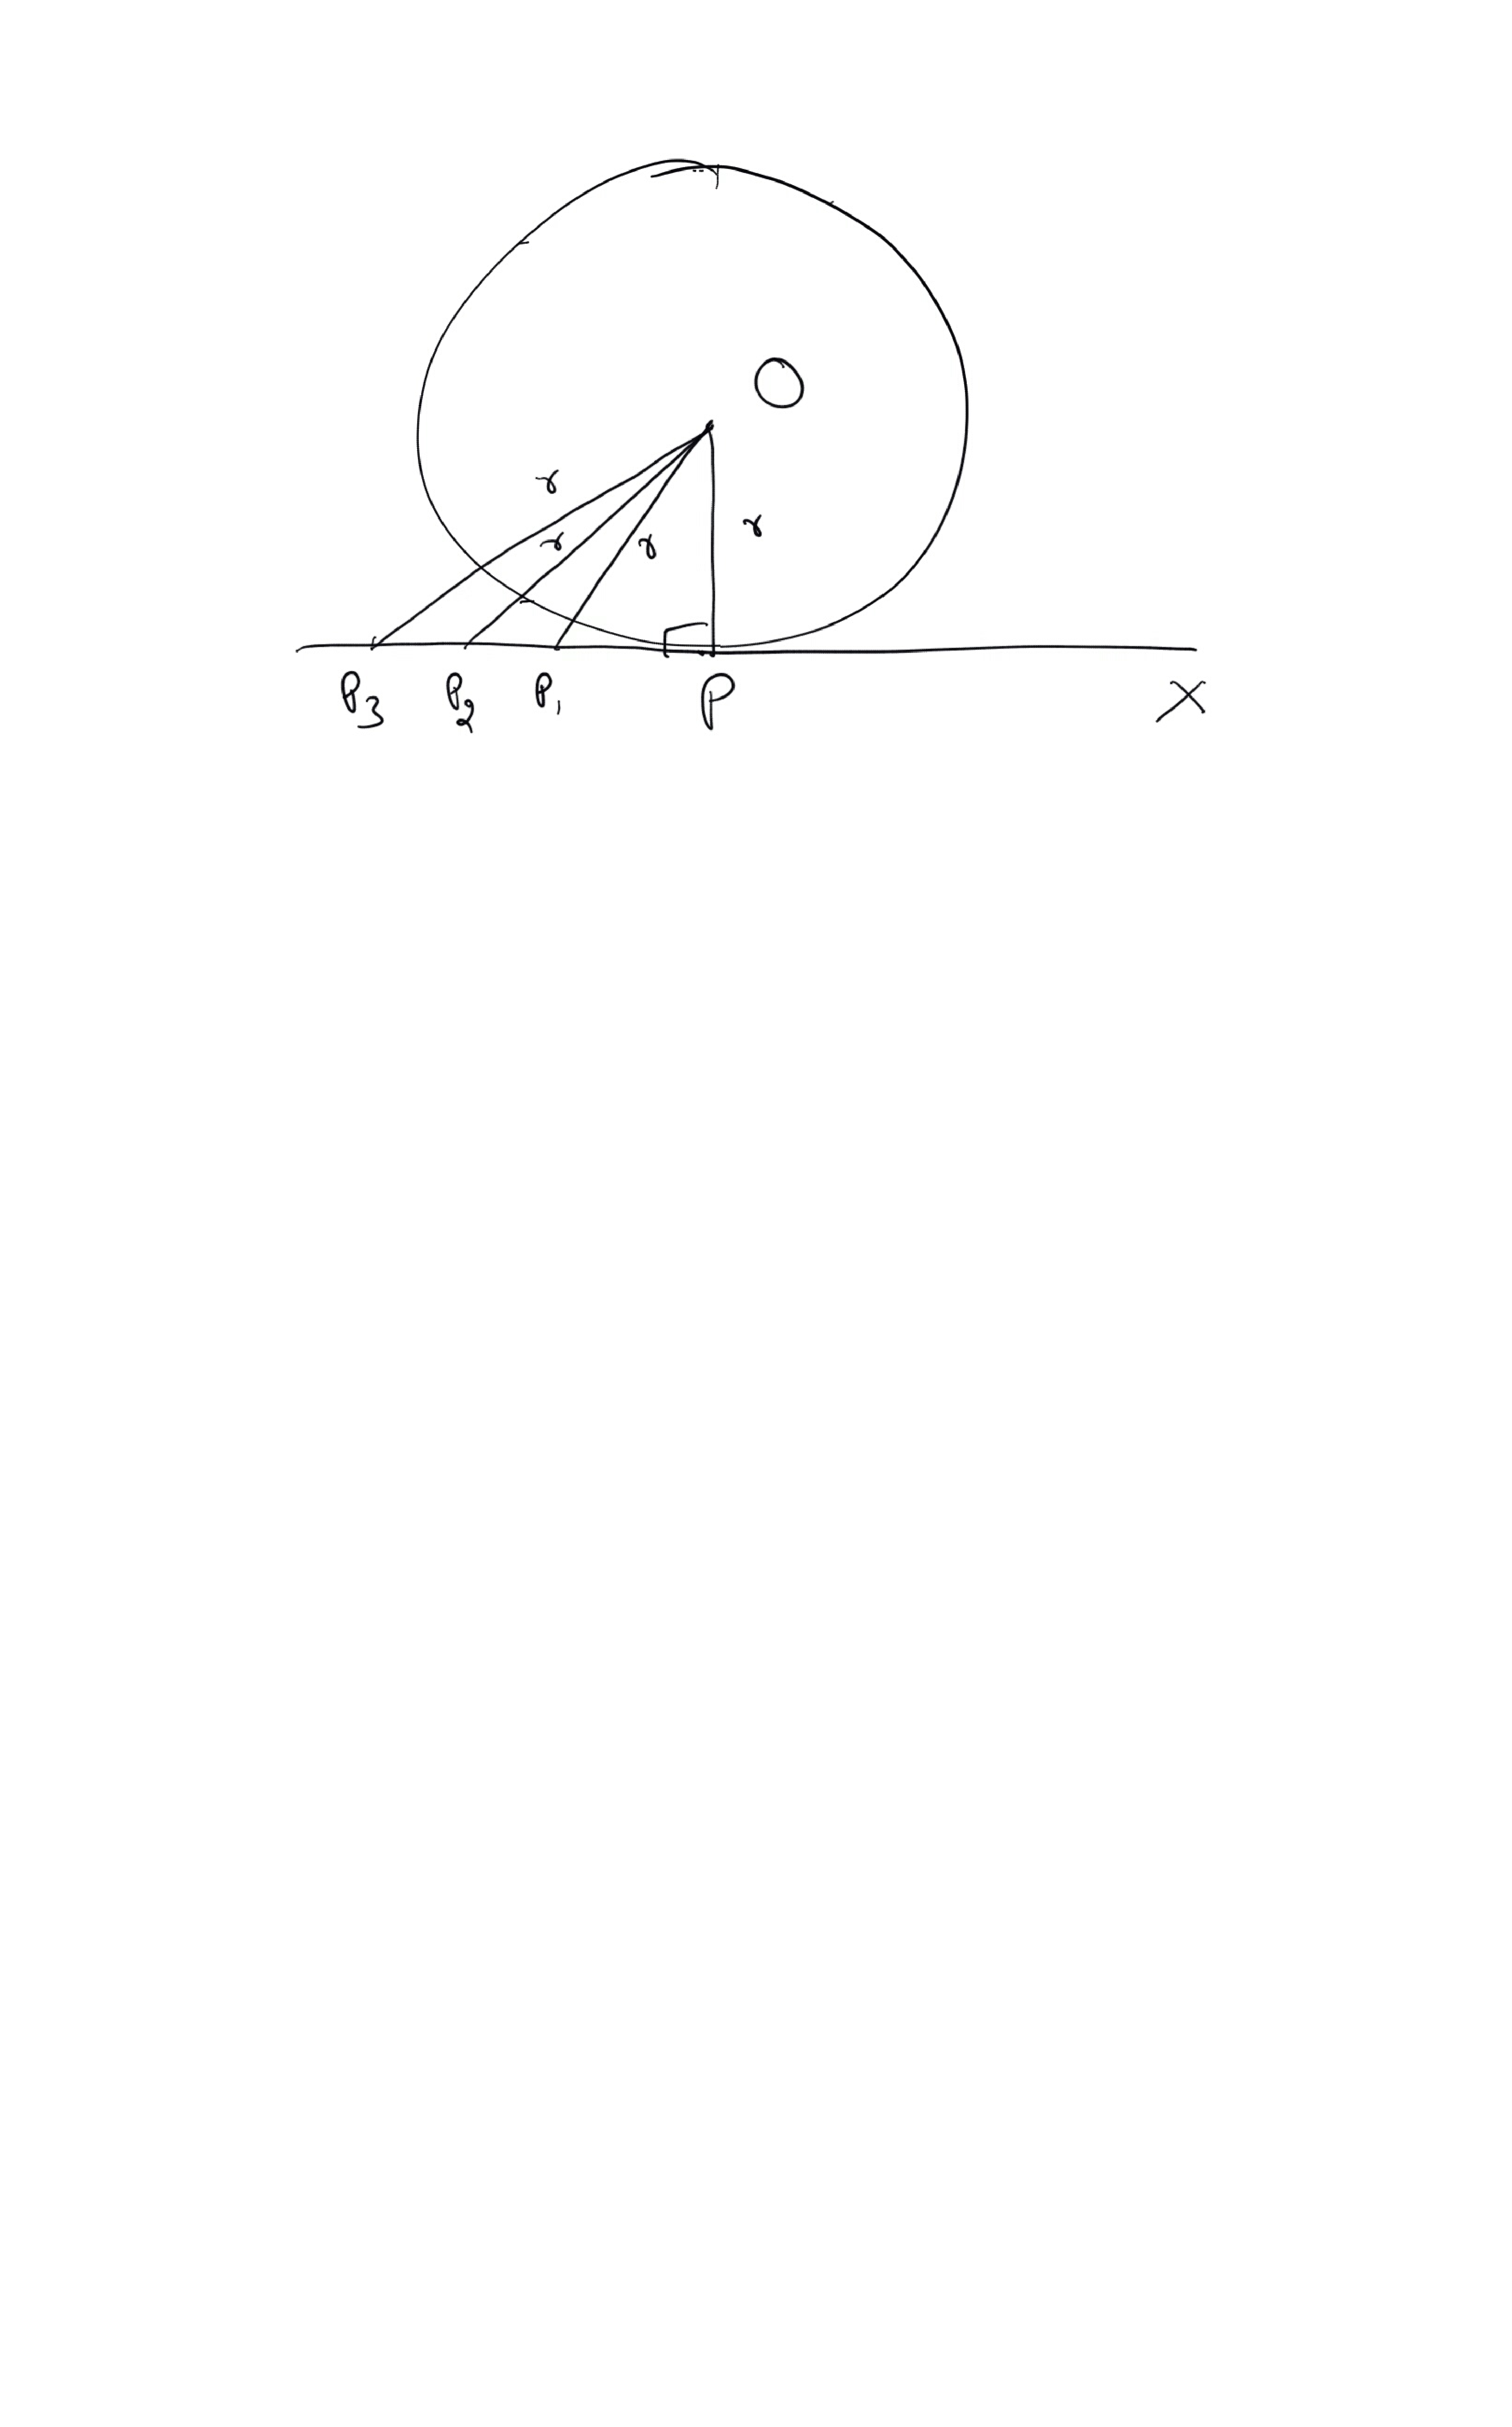
\includegraphics[width=\columnwidth]{./figs/ch4_tangent_def}
		\vspace*{-10cm}
	\end{center}
	\caption{Tangent to a Circle.}
	\label{ch4_tangent_def}	
\end{figure}
%
\begin{figure}[!h]
	\begin{center}
		
		
\includegraphics[width=\columnwidth]{./figs/ch4_short_dist}
		\vspace*{-10cm}
	\end{center}
	\caption{Shortest distance from $O$ to line $PX$}
	\label{ch4_short_dist}	
\end{figure}

%
\begin{equation}
\begin{split}
OP_1^2 &= OP^2 + PP_1^2 \\
\Rightarrow OP_1 > OP
\end{split}
\end{equation}
%
Thus, $OP$ is the shortest distance between $O$ and line $PX$.
%
\begin{problem}
Show that $\angle OPX = 90 ^{\degree}$
\end{problem}
\proof In Fig. \ref{ch4_tangent_def}, we can see that $OP$ is is the radius of the circle and the length of all line segments from $O$ to the line $PX > r$.  Using the result of the previous 
problem, it is obvious that $OP \perp PX$. 
%
	%
\begin{problem}
In Fig. \ref{ch4_tangent_prod} show that 
%
\begin{equation}
\angle PCA = \angle PBC
\end{equation}
%
$O$ is the centre of the circle and $PC$ is the tangent.
\end{problem}
	\begin{figure}[!h]
		\begin{center}
			
			
\includegraphics[width=\columnwidth]{./figs/ch4_tangent_prod}
			\vspace*{-10cm}
		\end{center}
		\caption{$PA.PB = PC^2$.}
		\label{ch4_tangent_prod}	
	\end{figure}
	%

%
\proof For convenience, greek letters are used for representing certain angles. Since $\Delta OAC$ is isosceles,
%
\begin{align}
2 \alpha + 2 \brak{\beta - \phi} &= 180^{\degree} \\
\Rightarrow  \alpha +  \brak{\beta - \phi} &= 90^{\degree} \\
\Rightarrow  \alpha +  \beta  &= 90^{\degree} + \phi
\end{align}
%
Since $theta$ is an exterior angle for the $\Delta ABC
$,
%
\begin{equation}
\theta = \alpha + \beta
\end{equation}
%
From both the above equations
%
\begin{equation}
\theta = 90^{\degree} + \phi
\end{equation}
%
Since PC is the tangent, 
%
\begin{equation}
\angle PCB = 90^{\degree} + \phi = \theta
\end{equation}
%
Considering the sum of angles in $\Delta PAC$ $\Delta PBC$,
%
\begin{align}
\angle P + \theta + \angle PCA &= 180^{\degree} \\
\angle P + \theta + \alpha &= 180^{\degree}
\end{align}
Hence,
%
\begin{equation}
\angle PCA = \alpha
\end{equation}
%
\begin{problem}
	In Fig. \ref{ch4_tangent_prod}, show that the triangles $PAC$ and $PBC$ are similar.
\end{problem}
\proof From the previous problem, it is obvious that corresponding angles of both triangles are equal.  Hence they are similar.
%
\begin{problem}
	Show that $PA.PB = PC^2$
\end{problem}
\proof Since $\Delta PAC \sim \Delta PBC$, their sides are in the same ratio.  Hence,
%
\begin{align}
\frac{PA}{PC} &= \frac{PC}{PB} \\
\Rightarrow PA.PB &=PC^2
\end{align}
%
%
\begin{problem}
	In Fig. \ref{ch4_chord_tangent_prod}, show that\begin{equation}
	PA.PB = PC.PD
	\end{equation}
\end{problem}
%
\begin{figure}[!h]
	\begin{center}
		
		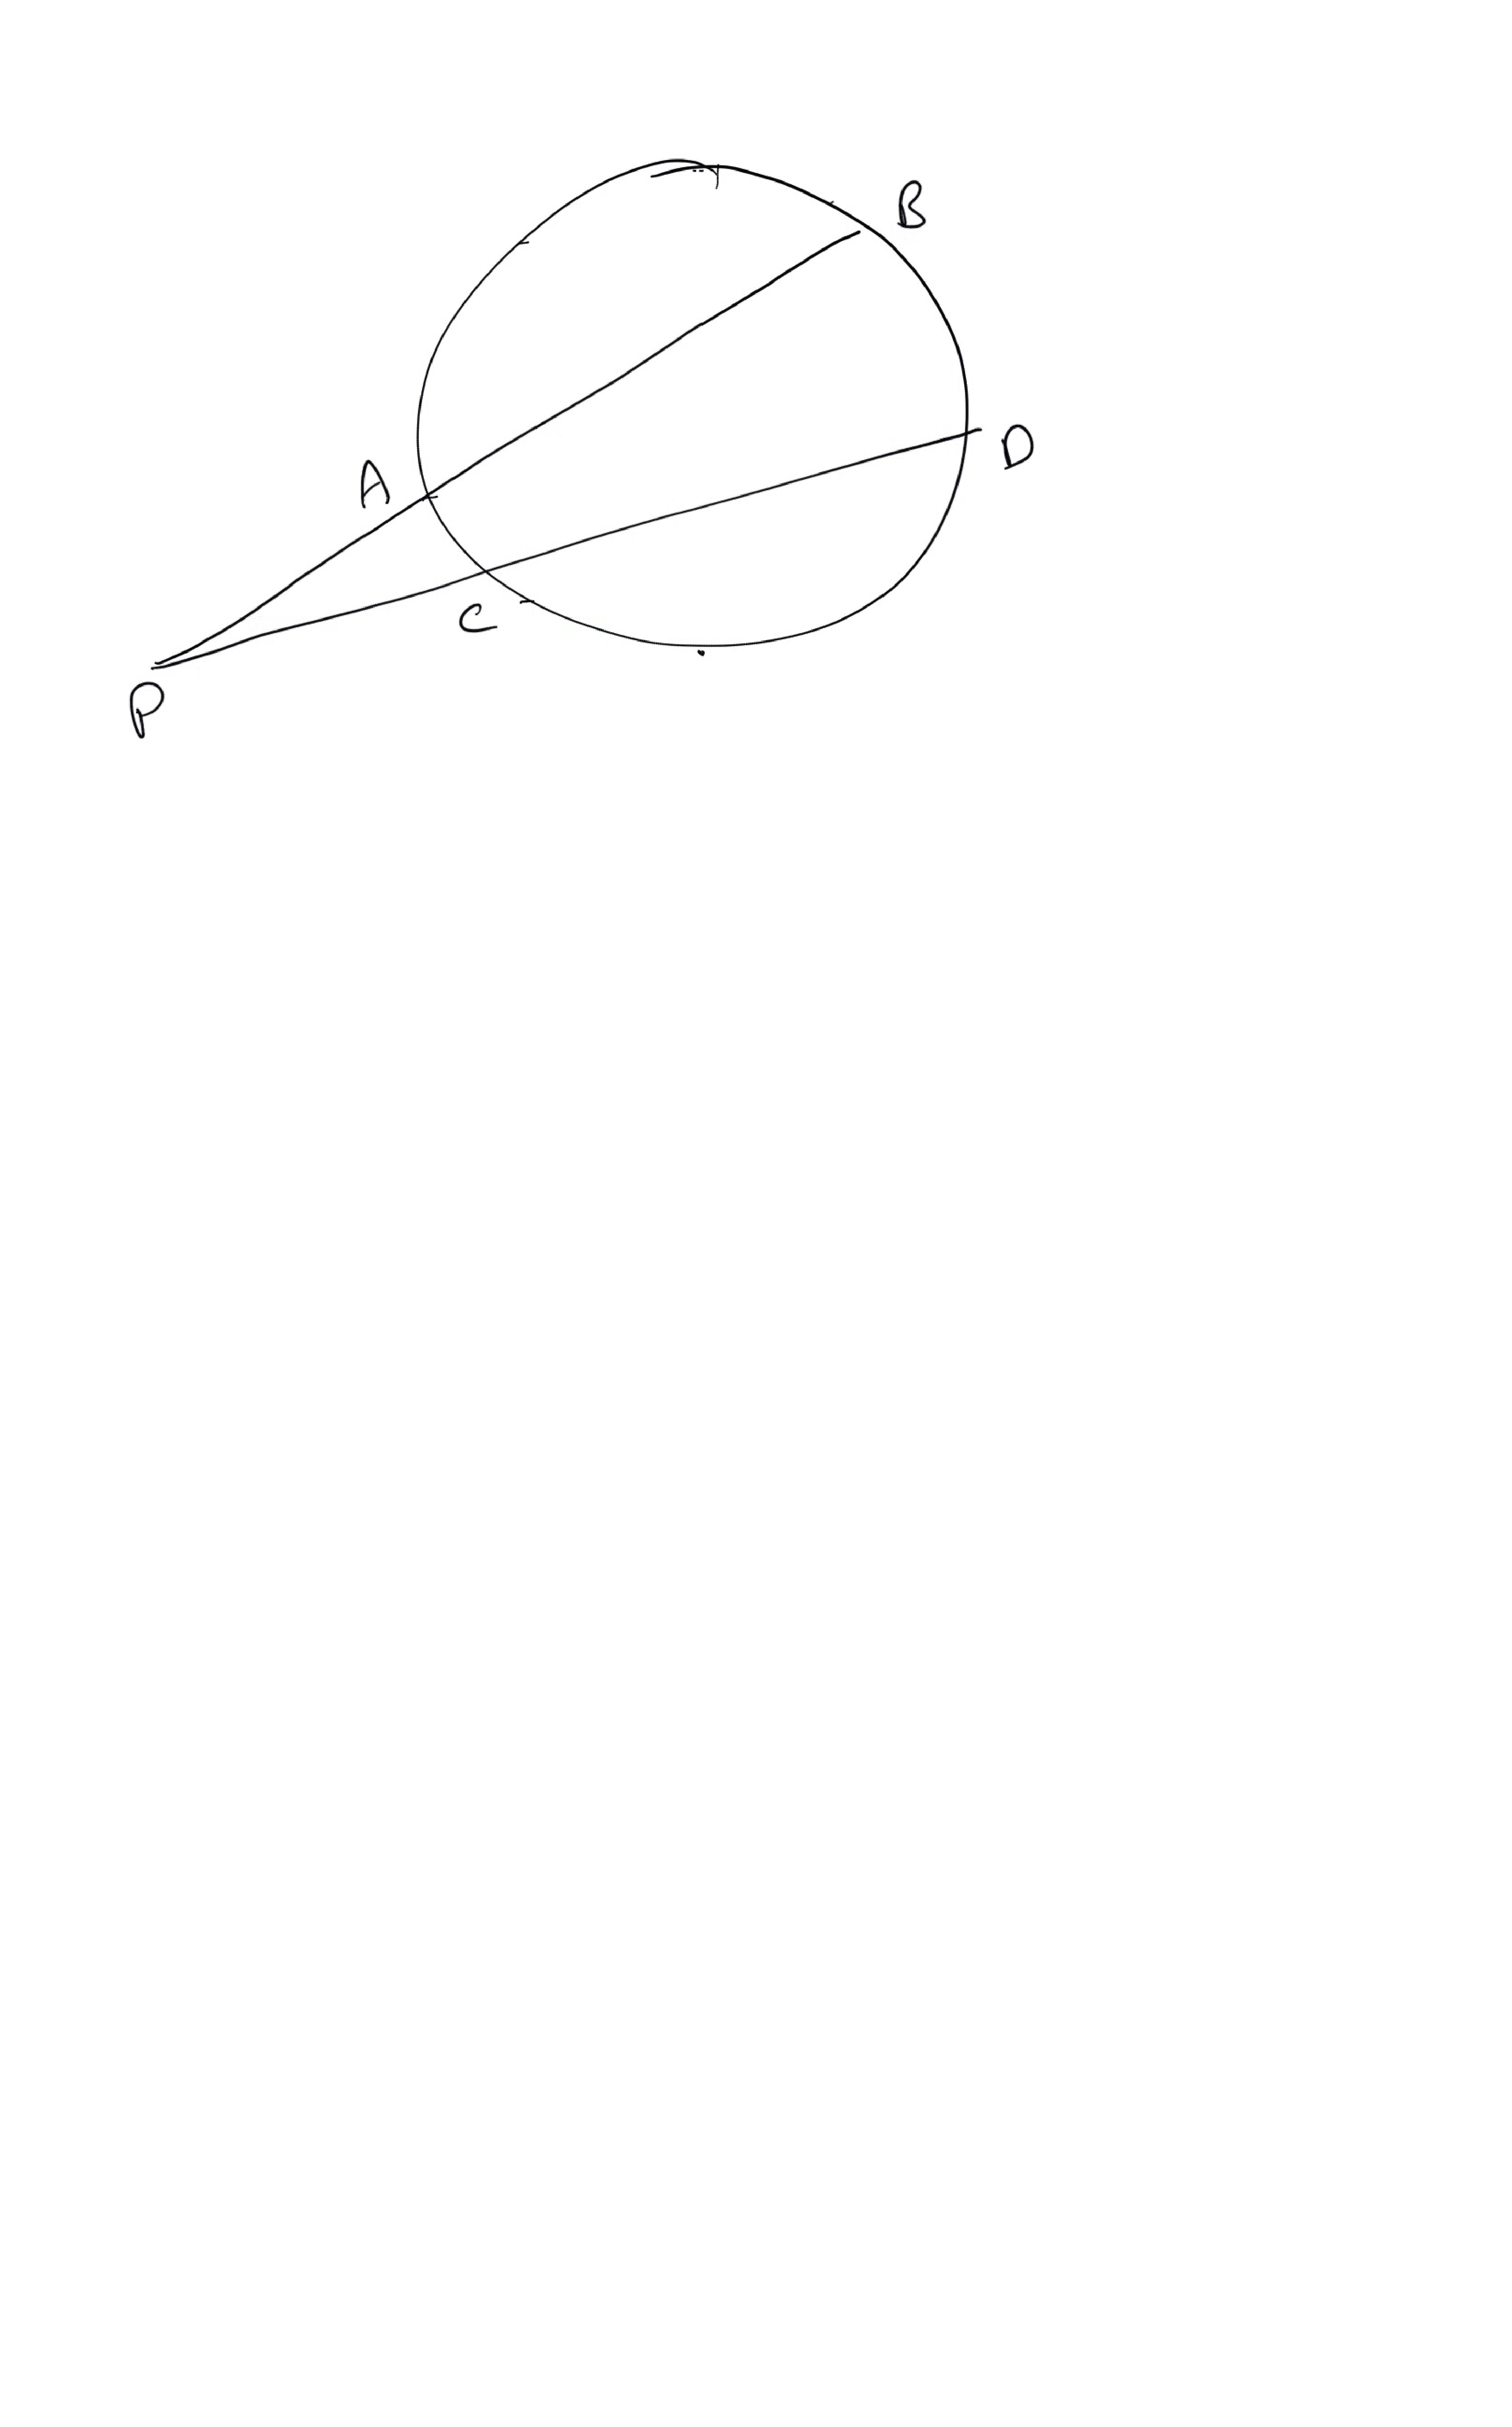
\includegraphics[width=\columnwidth]{./figs/ch4_chord_tangent_prod}
		\vspace*{-10cm}
	\end{center}
	\caption{$PA.PB = PC^2$.}
	\label{ch4_chord_tangent_prod}	
\end{figure}

\proof Draw a tangent and use the previous problem.
 




